\chapter{相关工作}

本文主要研究语言视觉激光多模态融合的机器人导航方法的研究及实现,研究方向是多模态融合的目标物体导航方法。
本章则主要介绍这个研究内容所设计到的技术,其中包括ROS系统及传感器间的通讯方法、联合标定、目标检测网络、多模态特征融合网络、点云聚类算法和PID控制器。


\section{ROS系统的通信与导航}
ROS(Robot Operating System)是一个运行于计算机操作系统上层开放源代码的机器人元操作系统,它提供了一整套灵活、模块化的通用框架,帮助工程师、研究人员和教育工作者等开发人员快速构建复杂的机器人系统。在经过开源机器人基金会(Open Source Robotics Foundation, OSRF)多年的精心维护和推广后,其社区活跃度、功能包丰富度、高扩展和高开发便利性上都表现十分出色,ROS已经成为机器人领域最流行的开发框架之一。

ROS系统主要由节点管理者(ROS Master)、话题(Topic)、发布者(Publisher)和订阅者(Subscriber)这四个部门共同组成,如图\ref{frossystem}所示。
\begin{figure}[htbp]
    \centering
    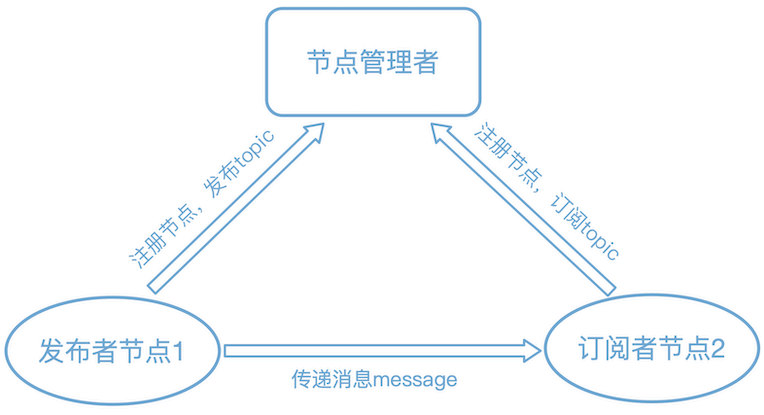
\includegraphics[scale=0.80]{Fig/rossystem.png}
    \caption{\label{frossystem}ROS系统组件图}
\end{figure}
其中,节点是ROS中的基本计算单元,负责执行如传感器数据采集、运动控制或算法处理等特定的任务,而一个完整的机器人系统通常由多个节点组成。话题是ROS中实现数据交换的核心机制。节点可以通过节点管理者发布消息到话题,或者通过订阅话题来接受消息,当订阅者想要获取某个特定发布者所发布的消息,只需要保证发布和订阅双方都监听同一个话题即可实现进程间的通讯。



在用户侧,ROS提供了一套机器人导航框架如图\ref{fROSNavstack}所示。该框架接收其它组件提供的地图、传感器信息、定位坐标关联、里程计信息,根据用户指定的导航目标点发布机器人执行的速度指令以运动到目标点。具体来说,ROS使用SLAM算法,通过获取传感器数据(如激光雷达或摄像头数据)和机器人运动信息来实时构建环境地图,然后,在创建的二维栅格地图的基础上,通过自适应蒙特卡洛(Adaptive Monte Carlo Localization, AMCL)等定位算法和传感器数据来实时估计机器人的位姿,最后,提供了move\_base作为导航框架主体,由局部、全局代价地图、全局规划期、局部规划期、失败恢复行为等组件来执行导航任务。

\begin{figure}[htbp]
    \centering
    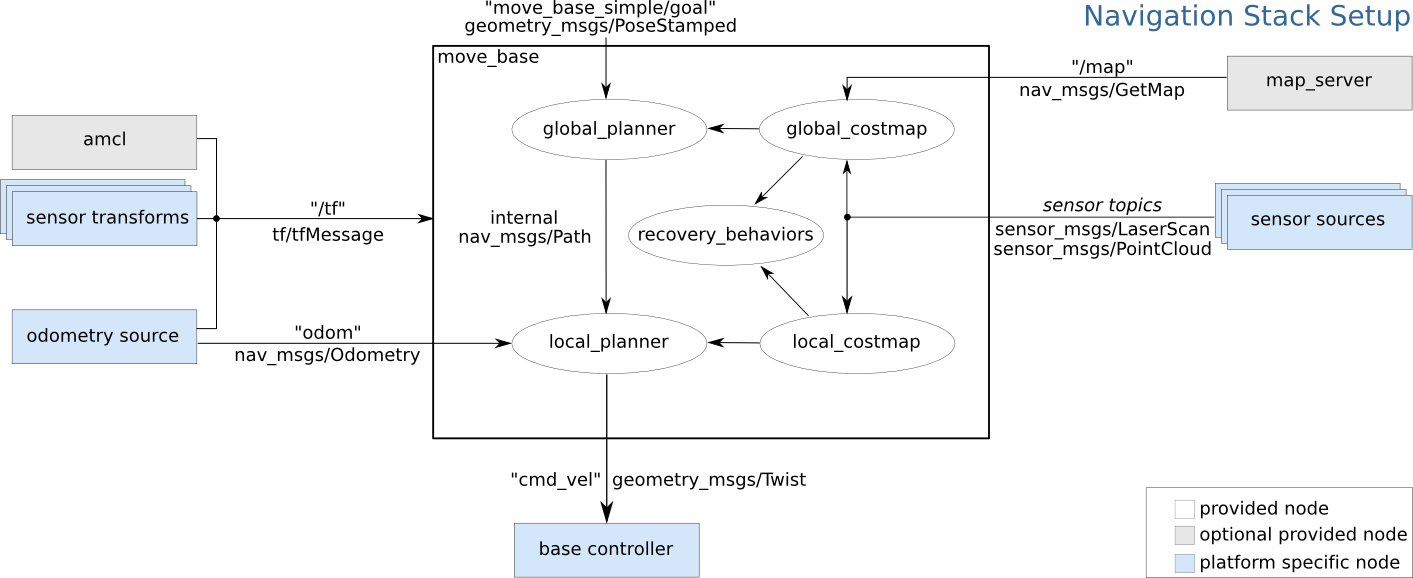
\includegraphics[scale=0.50]{Fig/ROSNavstack.png}
    \caption{\label{fROSNavstack}ROS导航框架图}
\end{figure}


除了上述的核心功能以外,ROS还提供了丰富的工具和生态系统,如可以实时显示机器人传感器数据、地图、路径等信息的可视化工具RViz、允许开发者在虚拟环境中测试机器人算法的高保真物理仿真环境Gazebo、用于记录机器人运行时的传感器数据工具ROS Bag,来帮助开发者更高效地开发和调试机器人系统。本文采用ROS系统的通信机制、导航方法和仿真环境来实现目标物体导航。


\section{联合标定}
在移动机器人上搭载的激光雷达和单目相机处于不同的坐标系之中,导致它们分别获取的点云数据和视觉图像信息无法直接一一对应起来,因此需要将这些传感器进行联合标定,以便于将点云数据映射到视觉图像中进行多模态融合。
本文使用张正友标定法\cite{zhang2002flexible}对激光雷达和单目相机进行联合标定,具体的过程如下图\ref{Calibration}所示。图中存在以单目相机的成像中心为原点的相机坐标系${\rm{Poin}}{{\rm{t}}_C} = {[{X_C},{Y_C},{Z_C}]^T}$、以激光雷达为原点的激光雷达坐标系${\rm{Poin}}{{\rm{t}}_L} = {[{X_L},{Y_L},{Z_L}]^T}$和以黑白棋盘格标定板的左下角为原点的世界坐标系${\rm{Poin}}{{\rm{t}}_W} = {[{X_W},{Y_W},{Z_W}]^T}$三个不同的坐标系。
\begin{figure}[htbp]
    \centering
    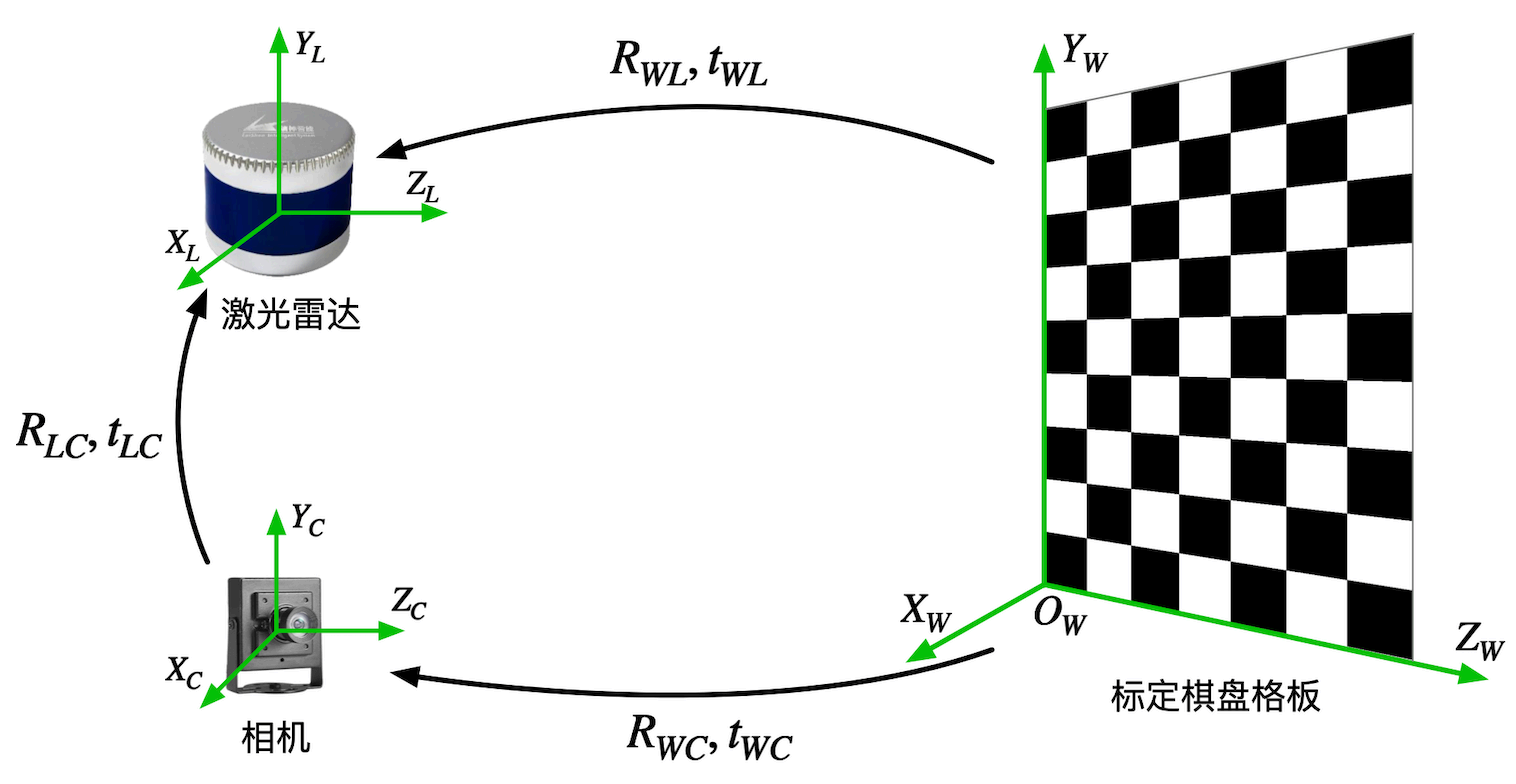
\includegraphics[scale=0.48]{Fig/joinCalibration.png}
    \caption{\label{Calibration}激光雷达和单目相机联合标定}
\end{figure}
联合标定就是要求解出一个用于翻转和平移坐标系的旋转矩阵和平移矩阵,即图中的${\rm{R}}_{LC}$和${\rm{t}}_{LC}$,使得激光雷达的点云能够映射到图像之中,将雷达感知到的物体与相机认知识别到的物体 对应起来。为此需要借助棋盘格标定板来求解它们直接的变换关系矩阵。

首先,相机坐标系中的三维坐标点${\rm{Poin}}{{\rm{t}}_C}$与像素平面上的二维坐标点${P_{uv}}$之间的转换关系可以表示为:
\begin{equation}
Z{P_{uv}} = Z\left[ {\begin{array}{*{20}{c}}
u\\
v\\
1
\end{array}} \right] = K\left[ {\begin{array}{*{20}{c}}
{{x_C}}\\
{{y_C}}\\
{{z_C}}
\end{array}} \right] = K \cdot {\rm{poin}}{{\rm{t}}_C}
    \label{myeq1}
\end{equation}

然后,在激光雷达坐标系下空间的任意一点都可以通过旋转矩阵${\rm{R}}_{LC}$和平移矩阵${\rm{t}}_{LC}$在另一坐标系中进行表示,它们之间的转换关系可以表示为:
\begin{equation}
{\rm{Poin}}{{\rm{t}}_C} = \left[ {\begin{array}{*{20}{c}}
{{x_C}}\\
{{y_C}}\\
{{z_C}}
\end{array}} \right] = {{\rm{R}}_{LC}} \cdot \left[ {\begin{array}{*{20}{c}}
{{x_L}}\\
{{y_L}}\\
{{z_L}}
\end{array}} \right] + {{\rm{t}}_{LC}} = {{\rm{R}}_{LC}} \cdot {\rm{Poin}}{{\rm{t}}_L} + {{\rm{t}}_{LC}} 
    \label{myeq2}
\end{equation}
将上式左项移动到右侧,变形可得:
\begin{equation}
    \delta \left( {{R_{LC}},{t_{LC}},{\rm{poin}}{{\rm{t}}_C},{\rm{poin}}{{\rm{t}}_L}} \right) = {R_{LC}} \cdot {\rm{poin}}{{\rm{t}}_C} + {t_{LC}} - {\rm{poin}}{{\rm{t}}_L}
    \label{myeq3}
\end{equation}

因此,借助棋盘格标定板可以在激光雷达和单目相机两个坐标系间获取多组互相匹配的特征点,进而使得上式中的$\delta \left( {{R_{LC}},{t_{LC}},{\rm{poin}}{{\rm{t}}_C},{\rm{poin}}{{\rm{t}}_L}} \right)$取得最小,即可得到旋转矩阵${\rm{R}}_{LC}$和平移矩阵${\rm{t}}_{LC}$,即:
\begin{equation}
    \left( {{R_{LC}},{t_{LC}}} \right) = \mathop {\arg \min }\limits_{{R_{LC}},{t_{LC}}} \frac{1}{2}{\sum {\left\| {\delta \left( {{R_{LC}},{t_{LC}},{\rm{poin}}{{\rm{t}}_C},{\rm{poin}}{{\rm{t}}_L}} \right)} \right\|} ^2}.
    \label{myeq4}
\end{equation}
上述非线性最小二乘方程可以使用Levenberg-Marquadt算法\cite{more1977levenberg}将其化成线性方程进行求解。获得的旋转平移矩阵将用于后续第四章的局部路径部分。



\section{目标检测网络}
在智能体进行自主导航的过程中,其搭载的算法模型通过视觉处理器对实时采集的视觉图像进行解析,从而获取包括各类物体的分类属性和空间坐标在内的特征参数。这些关键信息用于精准定位感兴趣的目标,并辅助智能体矫正可能出错的动作决策以逼近通向终点的最优路径。


目标检测的任务是从视觉图像之中认知并准确框出特定的目标物体,属于计算机视觉领域中需要解决的基础问题。与图像分类任务不同,目标检测不仅需要识别出图像中存在的物体类别,还需要精确地用锚框(Anchor)的形式定位出每个物体的位置信息及其对应的置信度分数。在早期还未出现基于深度学习的检测算法之时,开发者们大多都使用机器学习分类器\cite{viola2001rapid}或是依赖于人工设计的特征提取方法来实现初级的目标检测。但这类传统方法存在特征设计复杂、泛化能力有限等问题,难以应对复杂场景下的目标检测任务。

目标检测技术的发展与深度学习方法的更新迭代紧密相关,在卷积神经网络(Convolutional Neural Network,CNN)\cite{taye2023theoretical}主导的图像特征解析方法于公开数据集的目标检测竞赛中大放异彩后,这类技术方法迅速渗透到包括目标检测领域的各类人工智能算法之中并实现了革命性的突破,也逐渐形成了基于端到端思想的单阶段(One-stage)算法和基于区域生成的两阶段(Two-stage)算法这两大目标检测技术路线。

前者将目标检测任务视为一个统一的回归问题,一次性直接在图像上进行目标分类和锚框预测而不需要额外的区域生成步骤。
因此这类方法凭借这种端到端的结构更适用于实时目标检测的场景,能够有效满足工业级边缘设备对毫秒级响应时间的严苛需求,但在跟踪小物体或密集目标时效果较差。经典的One-stage目标检测模型包括:
\begin{enumerate}[topsep = 0 pt, itemsep= 0 pt, parsep=0pt, partopsep=0pt, leftmargin=44pt, itemindent=0pt, labelsep=6pt, label=(\arabic*)]
    \item 	YOLO\cite{redmon2016you}:早期YOLO系列的算法采用网格划分策略,它将输入图像分割成等尺寸的单元,让每个单元同时预测若干预设锚框的空间坐标、类别概率及置信度分数。在生成密集预测结果后,系统再通过非极大值抑制技术筛选最优边界框以去除冗余检测。这类方法的显著特点是检测效率高。得益于其单阶段检测架构,它无需区域建议等预处理步骤即可完成目标识别。然而,YOLO过于依赖非极大值抑制进行后处理以得到正确的检测框,这阻碍了其的端到端部署,并且对推理延迟产生了不利影响。除此之外,YOLO的各种组件设计缺乏全面深入的检查,导致明显的计算冗余,限制了模型的能力。与两阶段的目标检测算法相比,在面对小尺度目标或背景复杂的图像时YOLO的检测精度存在一定局限。
    \item	SSD\cite{liu2016ssd}:SSD通过预训练深度卷积主干网络在多个层级的特征空间中生成不同分辨率的特征映射,以此实现不同尺度大小物体的定位,但这种方法所使用的先验框参数十分依赖于人工预设,无法在训练过程中实现自适应调整,使得这类方法训练得出得模型泛化能力受限于参数调优策略,并且对小尺寸的目标识别效果仍然较差,存在特征提取不充分的情况。
\end{enumerate}

Two-stage算法将整个目标检测任务解耦为目标定位与目标识别两个阶段,首先通过区域生成网络(RPN)在特征提取层输出潜在得目标区域,接着在各候选目标区域进行类别判定和边界框回归以完成目标检测任务。Two-stage算法一般在正确率指标上会表现得更好,但其在检测时可能需要占用更多得资源、消耗更多的时间。代表性的Two-stage目标检测模型包括:
\begin{enumerate}[topsep = 0 pt, itemsep= 0 pt, parsep=0pt, partopsep=0pt, leftmargin=44pt, itemindent=0pt, labelsep=6pt, label=(\arabic*)]
    \item 	RCNN系列:包括RCNN\cite{girshick2014rich}、fastRCNN\cite{girshick2015fast}、FasterRCNN\cite{ren2016faster}等。这类算法的核心包括以下三点:1)通过区域生成网络(Region Proposal Network, RPN)在主干网络中的特征空间生成目标候选框;2)针对每个候选区域都会通过一个预训练的卷积神经网络进行特征提取,抑或是对每个候选区域使用RoI\cite{doukas2007region}池化进行固定大小的缩放;3)最后利用交叉熵损失函数与平滑L1损失共同优化分类置信度与边界框坐标参数。但这类方法存在检测实时性不足的问题。

    \item	基于Transformer:DETR\cite{carion2020end}是Transformer目标检测算法的开篇之作。它通过引入Transformer架构将目标检测过程视为一个由图形到集合的预测问题,消除了如锚框生成和非极大值抑制等后处理过程,通过二分匹配和一个转换器、编码器、解码器的结构和端到端的方式来进行目标的预测和类别的区分。但这类方法的训练时间长,模型的收敛速度慢,且在小物体的检测时性能较差。
\end{enumerate}

\begin{figure}[htbp]
    \centering
    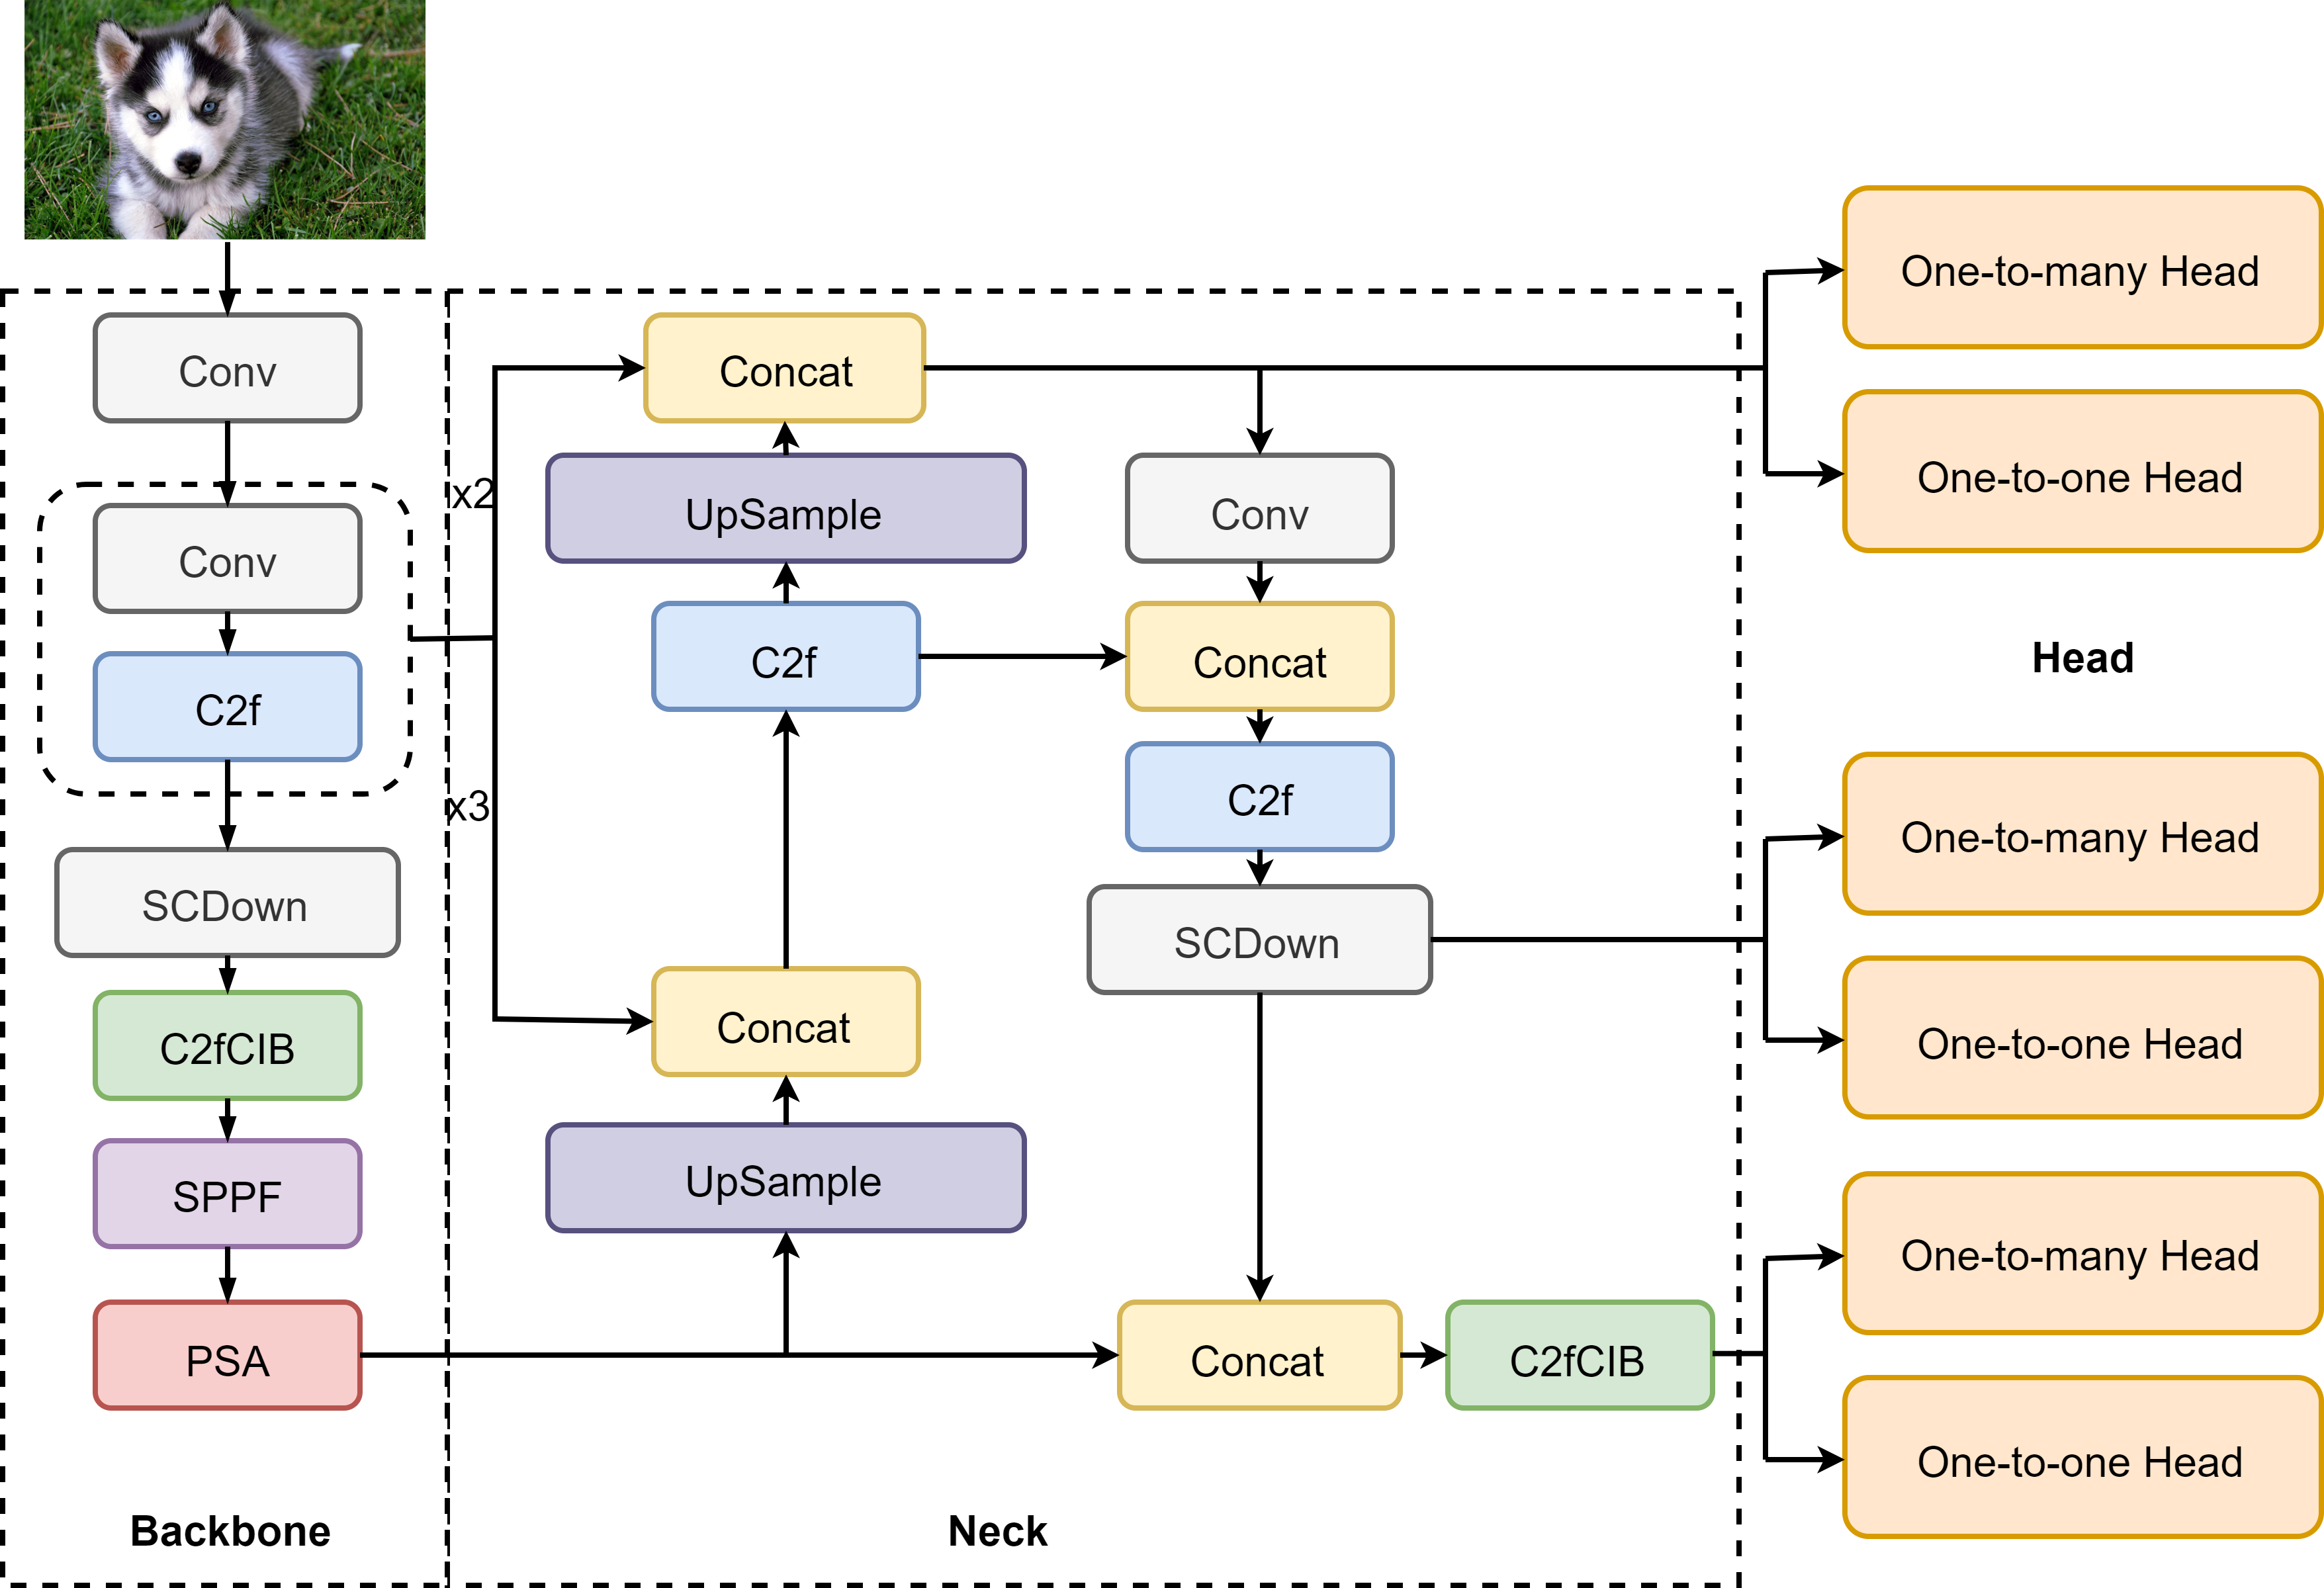
\includegraphics[scale=0.12]{Fig/yolonet.png}
    \caption{\label{fyolonet}YOLOV10网络}
\end{figure}

为了满足整个导航过程中目标检查所需的实时性和可靠性,本文使用的目标检测网络是YOLOV10网络\cite{wang2025yolov10},如图\ref{fyolonet}所示。YOLOV10与YOLOV8\cite{varghese2024yolov8}相比在整体的网络结构上基本保持一致,网络分为骨干网络(Backbone)、颈部(Neck)、头部(Head)三个部分。首先将图片输入骨干网络中提取图像的全局和局部特征,在颈部通过Upsampling、Concat和注意力机制卷积网络增强特征的表达能力,实现有效的特征提取和融合,并在头部将颈部提取的特征映射到最终的输出空间,生成网络的最终预测结果。然而,相较于后者,YOLOV10为了实现更加轻量化的端到端部署而做出了几点重要的优化:
\begin{enumerate}[topsep = 0 pt, itemsep= 0 pt, parsep=0pt, partopsep=0pt, leftmargin=44pt, itemindent=0pt, labelsep=6pt, label=(\arabic*)]
    \item 	轻量化分类头(Lightweight Classification Head):在YOLOV8网络结构中Head部分的分类头的参数量和计算量比回归头更大,但后者对检测精度的影响更大,因此减少分类头的卷积参数量以达到轻量化模型的目的。
    \item	空间-通道分离下采样(Spatial-Channel decoupled downsampling, SCDown):YOLOV8使用一个标准卷积时实现空间下采样和通道变换,SCDown将这两种操作进行解耦,先通过逐点卷积调节通道维度,然后通过深度卷积进行空间下采样,保证降低计算成本的同时最大限度保留信息。
    \item   精度驱动的模型设计:在小模型规模的深层阶段使用大核卷积(Large-kernel Conv)来扩大感受野,增强模型能力;针对计算开销过大的自注意力机制设计了一种高效的部分自注意力(Partial self-attention, PSA),对分辨率最低的特征的一半进行计算,将对于全局的学习能力以较小的计算成本融入到网络中。通过这些方法可以在不显著增加计算成本的情况下提升模型的性能。
    \item   基于秩的块设计:YOLOV10使用了一种分层特征优化的紧凑反转模块(CIB)结构,它通过低复杂度的深度卷积方法来实现局部空间的特征融合,同时结合轻量化的点卷积操作完成跨通道信息交互,这一设计有效缓解了传统检测模型中由同构模块堆叠所引发的参数冗余问题。
\end{enumerate}


\section{多模态特征融合网络}

多模态特征融合是指通过整合多种来源或不同形式的数据信息来训练一种能够提升系统认知能力或执行效果的技术,这种技术旨在充分发挥各模态间的优势互补特性从而提升系统在模式辨识、类别划分和内容生成等任务中的表现能力。

在机器人执行导航任务的探索阶段将采用特征融合框架对异构感知信息进行融合,通过语义编码器提取的文本描述特征、目标物体识别算法提取的语义局部信息、深度卷积模型提取的环境特征来得到可以指导机器人进行局部导航的动作决策。现阶段的多模态融合方法按照融合的阶段的不同可以分为以下三种类型:
\begin{enumerate}[topsep = 0 pt, itemsep= 0 pt, parsep=0pt, partopsep=0pt, leftmargin=44pt, itemindent=0pt, labelsep=6pt, label=(\arabic*)]
    \item 	特征级融合:这种融合方法是在神经网络的核心处理模块之前,通常是在数据输入环节,将多种模态的特征进行整合。比如,在数据输入阶段就将视觉信息和文本信息进行融合。
    \item	模型级融合:这种融合方式选择在神经网络的中间层级进行多模态信息的整合。具体做法可以是将各模态经过独立学习后的特征表示进行合并,然后再进行后续的网络处理。
    \item	决策级融合:该策略在完成各模态的独立处理后在决策或输出层进行融合。在每个模态的数据都经过单独处理后,通过将各模态的输出结果进行融合以形成最终决策。这种方法的优势在于其灵活性高且能兼容经过预训练的单模态模型。
\end{enumerate}

本文将采用第三种融合方法,即使用Transformer网络进行后期的决策级融合,Transformer网络的操作流程如图\ref{ftransformer}所示。Transformer网络的核心创新在于采用了多头自注意力机制\cite{niu2021review}。自注意力的核心原理是通过计算序列中各元素间的关联度来生成相应的注意力权重,再基于这些权重对序列元素进行加权整合从而达到自注意的目的。多头机制则通过并行使用多个注意力单元使每个单元能够学习到不同的权重分布,从而让模型能够在多个特征子空间中对输入序列进行多样化表征。这种设计方法使Transformer能够突破传统模型的局部窗口限制来实现对序列全局信息的有效捕捉。多个注意力单元可以分别聚焦于不同类型的信息特征,这样可以显著增强网络在处理多模态数据时的特征融合能力。具体来说:
\begin{equation}
    \begin{array}{c}
Attention\left( {Q,K,V} \right) = softmax\left( {\frac{{Q{K^T}}}{{\sqrt {{d_k}} }}} \right)V\\
hea{d_i} = Attention\left( {QW_i^Q,KW_i^K,VW_i^V} \right)\\
MultiHead\left( {Q,K,V} \right) = Concat\left( {hea{d_1}, \ldots ,hea{d_n}} \right){W^O}
\end{array}
    \label{myeq7}
\end{equation}
其中,查询($Q$)、键($K$)和值($V$)由输入序列通过三个线性变换获得的矩阵,$W_i^Q$、$W_i^K$和$W_i^V$分别是$Q$、$K$和$V$的权重矩阵,${d_k}$表示特征维度,$hea{d_i}$表示第i个注意力头,${W^O}$表示连接多个注意力头输出的权重矩阵Attention表示子注意力机制,MultiHead是多头自注意力机制。
\begin{figure}[htbp]
    \centering
    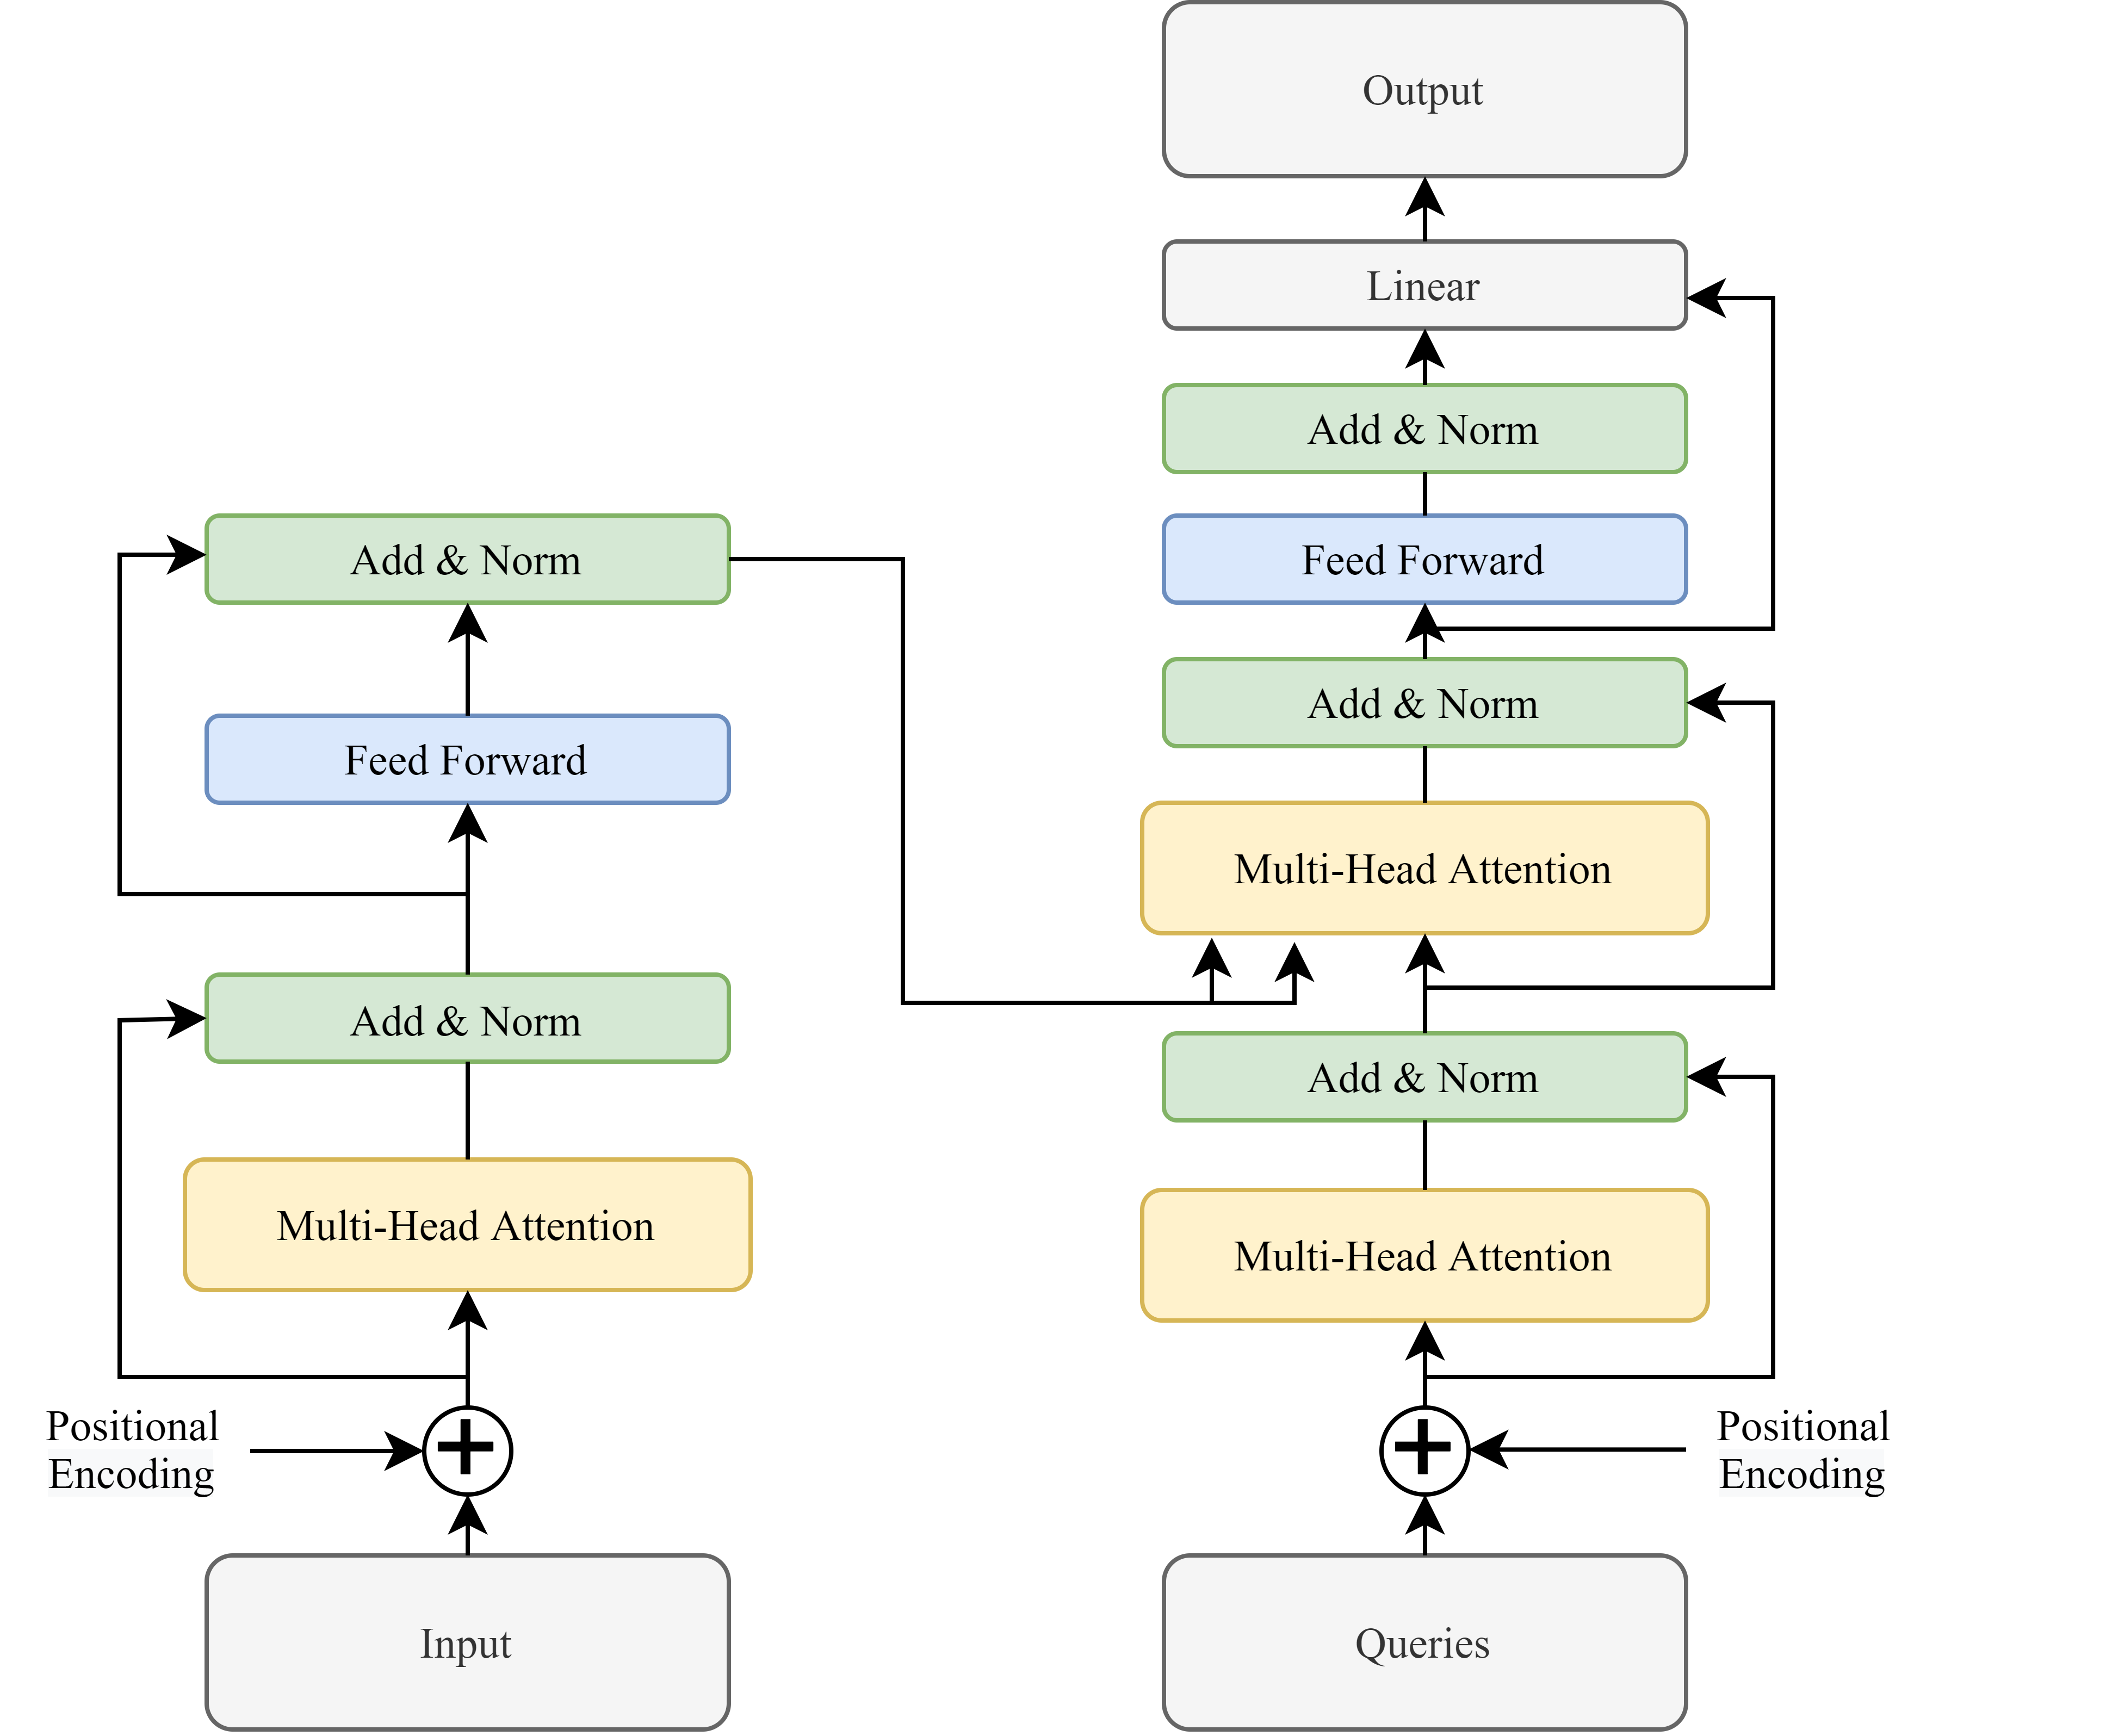
\includegraphics[scale=0.10]{Fig/transformer.png}
    \caption{\label{ftransformer}Transformer网络结构}
\end{figure}

\section{点云聚类}
三维激光雷达获取的点云具有精度高、空间坐标信息准确的特点,因此在移动机器人的导航过程中常用于实时定位与环境感知,但点云数据是一种非结构化的离散数据,在环境感知的过程中需要通过高效的聚类算法来区分从属于不同目标的点云。目前主流的聚类方法一般会使用基于局部表面曲率、法向量方向这类几何属性与密度梯度、高程变化这类空间分布特征进行特征编码,便于将点云映射至可聚类特征域,欧式聚类就是这类算法的典型例子,它通过KD-Tree加速邻域搜索实现O(n*logn)级时间复杂度的快速点云分割,但也需要根据雷达点云近密远稀的特性对距离阈值进行动态调整。针对不同的应用场景还存在密度聚类、超体聚类等算法,它们在耗时和聚类准确率方面各有优势。在目标物体导航的过程中要求系统需要更强的实时性,因此本文采用欧式聚类\cite{liu2021point}方法对三维点云进行预处理。


欧式聚类法在点云密集的情况下需要进行额外的优化以保证其实时性,这里采用点云栅格化和kd树对算法进行加速优化\cite{guo2023kd}。栅格化方法首先将扫描区域划分为若干网格单元,将三维点云投影至二维平面,保持z轴数值不变的同时,将每个网格内点的x、y坐标统一为该网格中心点坐标。随后进行去重处理,对于x、y坐标相同且z值相近的点只保留一个代表性点,通过栅格化方法对点云数据进行处理能够显著减少计算复杂度。除此之外,本文利用PCL库中的KdTree->setInputCloud()函数将栅格化后的点云构建为k维二叉树结构,借助kd树结构优化近邻搜索过程,进一步提升欧式聚类算法的效率,本文改进的欧式聚类算法的伪代码见Algorithm\ref{algorithm1}。
\begin{algorithm}[!h]
    \caption{可变距离阈值的欧式聚类算法}
    \label{algorithm1}
    \renewcommand{\algorithmicrequire}{\textbf{Input:}}
    \renewcommand{\algorithmicensure}{\textbf{Output:}}
    \renewcommand{\algorithmiccomment}[1]{\hfill $\triangleright$ #1}
    \begin{algorithmic}[1]
        \REQUIRE 激光点云$P$  %%input
        \ENSURE 点云蔟集合$C$    %%output
        \STATE  对激光点云$P$进行栅格化和kd树预处理;
        \STATE  创建点云蔟列表$C$
        \STATE  创建当前点云蔟$c$
        \FOR{${p_i} \in P$}
            \STATE  que.push(${p_i}$)
            \COMMENT{遍历点云$P$中的每个点,并将当前点${p_i}$加入队列}
            \WHILE{!que.empty()}
                \STATE  ThresholdGet(${p_i}$)$ \to {d_{th}}$
                \COMMENT{计算当前点对应的距离阈值}
                \STATE  KdtreeSearch($P$,${p_i}$,${d_{th}}$)$ \to P_i^k$
                \COMMENT{使用kd树寻找${p_i}$的邻近点}
                \FOR{${p_j} \in P_i^k$}
                    \STATE  que.push(${p_j}$)
                    \COMMENT{遍历${p_i}$的临近点,并将其加入队列中}
                \ENDFOR
                \STATE  $c = c \cup {p_i}$
                \COMMENT{将找到的这簇点云加入结果集中}
                \STATE  que.pop()
            \ENDWHILE
            $c = \emptyset $
        \ENDFOR
    \end{algorithmic}
\end{algorithm}

距离阈值是用来区分不同簇点云的重要参数,当设定的距离阈值${d_{th}}$小于一个点集${P_m} = \left\{ {{p_m} \in P} \right\}$与另一个点集${P_n} = \left\{ {{p_n} \in P} \right\}$之间的最小距离,则可以判定这两个点集为两簇不同的点集。因此点云簇为两簇不同的点云的条件可以表示为
\begin{equation}
    \min \left\| {{p_m} - {p_n}} \right\| \ge {d_{th}}
    \label{myeq5}
\end{equation}

近密远稀是激光雷达这类设备的共同特点,表现为空间中点云的密度会随着其与原点的距离的减小而逐渐增加、增加而逐渐减小,如图\ref{fcarpoints}所示,随着车辆与激光雷达之间的距离增大,其反射生成的点云分布密度显著降低。传统的欧式聚类算法依赖于固定的距离阈值来划分障碍物,这种方法难以应对点云密度随距离变化的情况。本文通过调整距离阈值参数设计了一种自适应的欧式聚类方法来解决空间点云发散而导致聚类效果不好的问题,如\eqref{myeq6}所示,距离阈值参数$d_{th}$会随着点云与原点距离的增大而逐渐增大。

\begin{figure}[htbp]
    \centering
    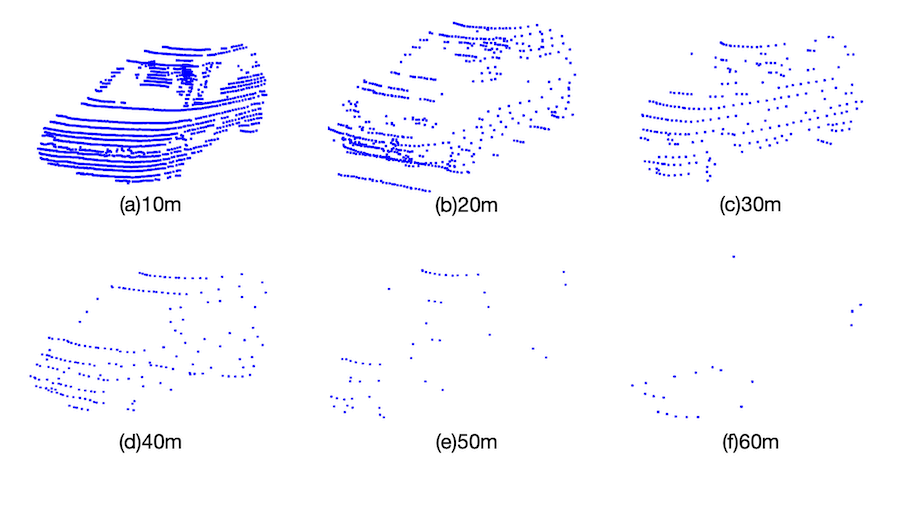
\includegraphics[scale=0.75]{Fig/carpoints.png}
    \caption{\label{fcarpoints}障碍物点云随着距离增加变稀疏}
\end{figure}
\begin{equation}
    {d_{th}} = \left\{ {\begin{array}{*{20}{c}}
{5cm}\\
{10cm}\\
{15cm}\\
{20cm}
\end{array}} \right.{\rm{ }}\begin{array}{*{20}{l}}
{0 < Range \le 1.5m}\\
{1.5m < Range \le 3.0m}\\
{3.0 < Range \le 5m}\\
{5m < Range}
\end{array}
    \label{myeq6}
\end{equation}
本文使用的十六线激光雷达在不同距离的聚类测试中表现出明显的波动,当雷达与目标之间的距离超过5米后z轴方向的点云密度衰减十分严重,聚类的可靠性明显下降,因此我们在自适应方法中添加了终止机制,即$d_{th}$在5m后的范围不再迭代更新。

点云聚类算法的结果用于后文第四章所介绍的点云映射中,将点云感知信息与图像认知信息的结果相融合,以获得目标检测算法认知到的目标物体的精确位置信息。

\section{PID控制器}

PID控制器是一种广泛使用的反馈控制系统,能够根据目标值与当前值之间的偏差来调整控制变量,从而使系统稳定地达到设定目标。具体而言,PID控制器通过调节比例、积分和微分来控制机器人的运动,确保其到达预定的位置或保持稳定的姿态,如图\ref{pid},它简单易用,适用于大多数线性控制问题,具有很好的实时性和鲁棒性。
\begin{figure}[htbp]
    \centering
    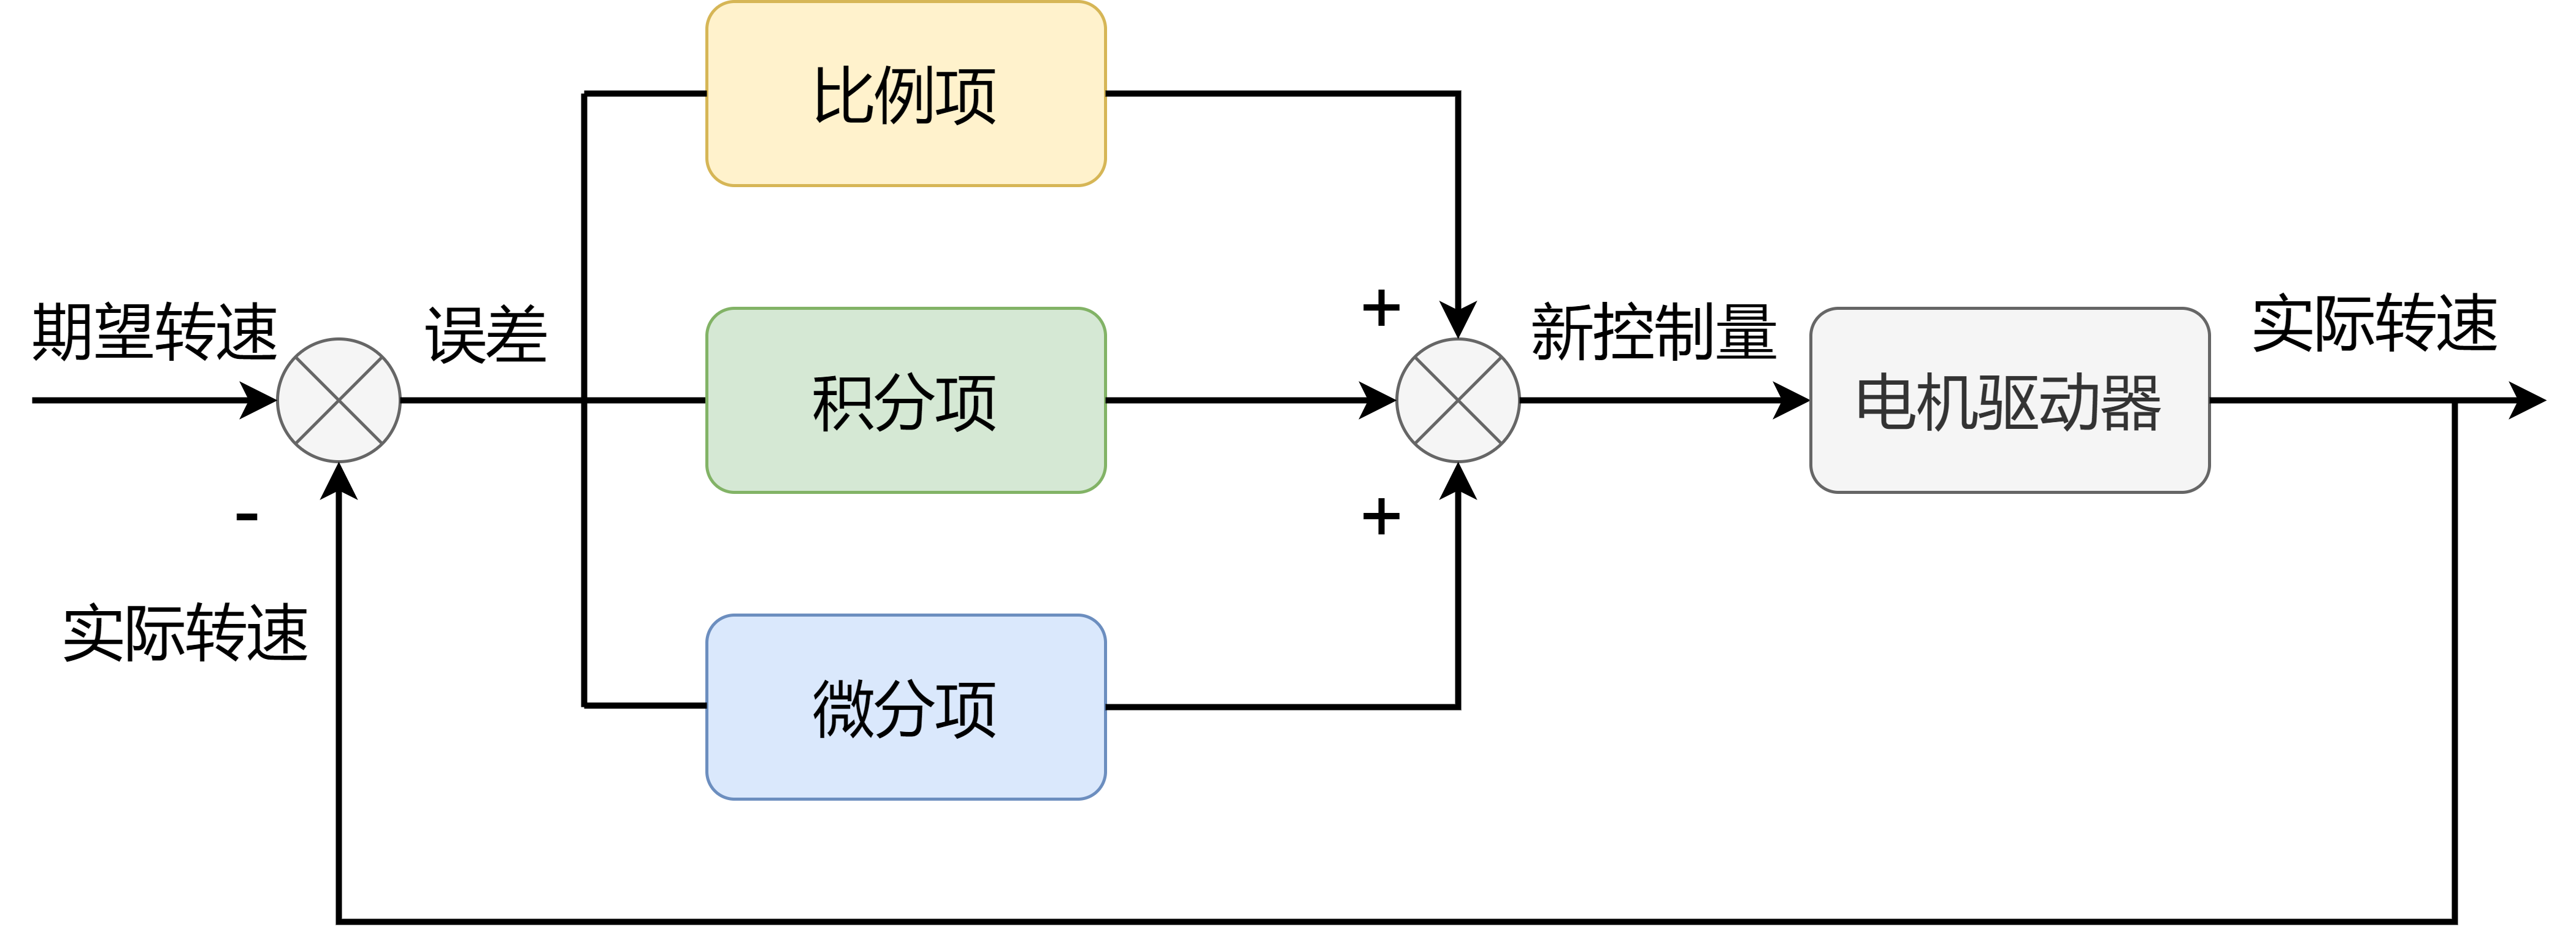
\includegraphics[scale=0.06]{Fig/pid.png}
    \caption{\label{pid}PID算法控制电机转速}
\end{figure}

比例项是PID控制器中最基础的组成部分,它直接根据期望值与实际值之间的偏差来进行调整,如式\ref{myeq17},其中$P$表示比例控制输出,${K_p}$表示比例增益,即在误差变化时控制器输出的变化幅度,$e\left( t \right)$表示当前时刻的误差,当误差越大时,比例项的输出也就越大,以帮助系统更快速的接近目标值。
\begin{equation}
    P = {K_p} \cdot e\left( t \right)
    \label{myeq17}
\end{equation}

积分项是PID控制器中的第二个组成部分。积分项的目的是消除系统在长时间运行中可能出现的静态误差,确保系统达到并保持在期望的目标位置,如式\ref{myeq18},其中$I$表示积分控制输出,${K_i}$表示积分增益,能够决定积分项对控制输出的影响程度,${e\left( t \right)}$表示误差。当系统的输出长期无法达到设定的目标时,积分项就会逐渐地累积来弥补系统长期积累的偏差,一直到该误差消除。
\begin{equation}
    I = {K_i} \cdot \int_0^t {e\left( t \right)dt} 
    \label{myeq18}
\end{equation}

当积分增益过大时会导致系统响应过度,引发系统的超调和震荡,这时候就需要通过微分项来预测误差的变化趋势以减少系统发生超调和震荡的可能。与前面介绍的两者不同,微分项主要关注的是误差变化的速度而非当前的误差值,如式\ref{myeq19},其中$D$表示微分控制输出,${K_d}$表示决定了微分项对控制输出的影响程度的微分增益,$\frac{d}{{dt}}e\left( t \right)$表示用来预测未来误差变化趋势的误差变化速率。通过微分项的预测误差和提前调整,系统能够避免震荡和过调现象的发生,让系统更加平稳的响应。
\begin{equation}
    D = {K_d} \cdot \frac{d}{{dt}}e\left( t \right)
    \label{myeq19}
\end{equation}
通常情况下积分项、比例项和微分项会一起使用,即通过比例项消除实时误差,利用积分项来消除长期累计的误差,而微分项则通过对误差变化率的敏感度调整来预测误差的变化趋势,减少系统发生超调和震荡的概率,三者相辅相成一同构成一个完整的PID控制器,使其能够更精准、更平稳地调节系统响应。

PID控制器将用于后文第四章所介绍的运动模块中,以执行特征提取、融合模块所输出的导航动作。

\section{本章小结}
本章主要内容是目标物体导航过程中涉及到的一些常用的算法原理和关键技术,主要介绍了ROS系统及传感器间的通讯方法、联合标定、目标检测网络、多模态特征融合网络、点云聚类算法和PID控制器。

